\subsection{Input Files and Distributed Storage}
\label{sec:input_file_gathering}

\begin{figure}
  \centering
  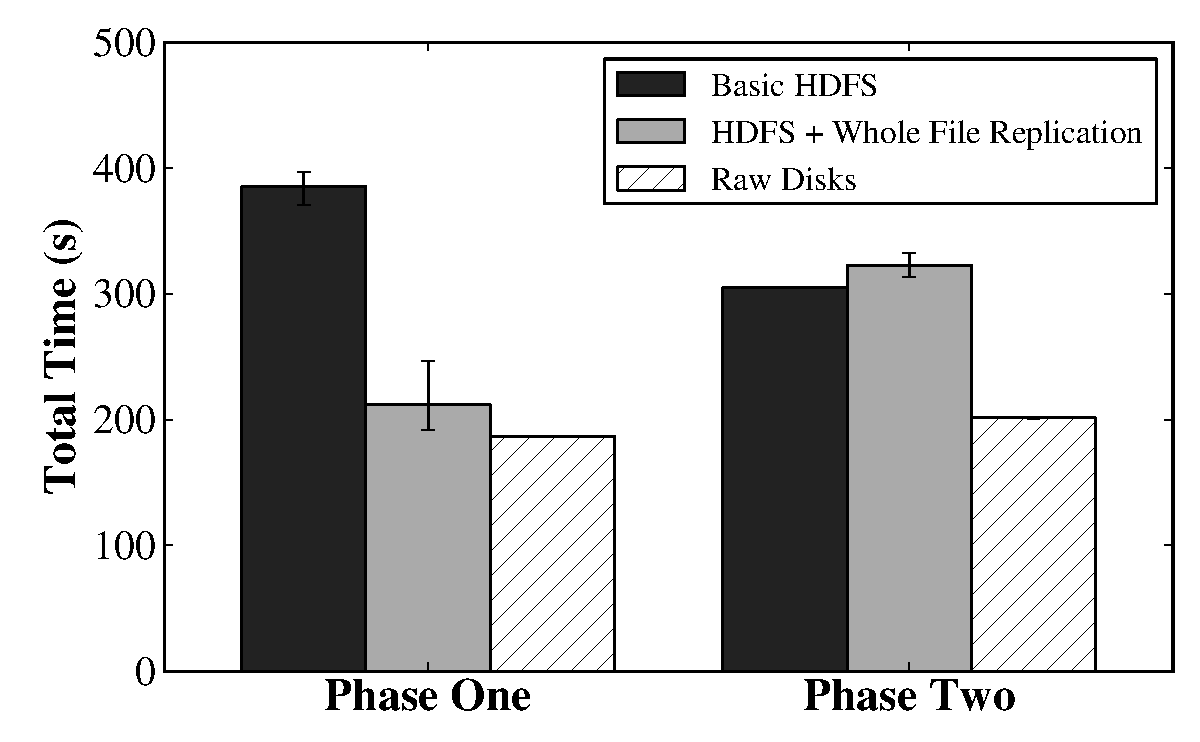
\includegraphics[width=\columnwidth]{fault_tolerance/graphs/hdfs_no_proxy_penalty}
  \caption{\label{fig:hdfs_no_proxy_penalty} Comparing the performance of
    unmodified HDFS, HDFS with whole file replication for the primary replica,
    and reading and writing from raw disks.}
\end{figure}

The specification of each \themis job includes an input directory; all files in
the input directory are processed. \themis can read input files from raw disks
or from HDFS~\cite{hdfs} using the WebHDFS REST API. We use HDFS exclusively in
this work.

Each file is uniquely identified by its URL, which is of the form\\
\texttt{<protocol>://<host>:<port>/<path from root>}. Each file is also given a
file ID that must be unique within the job. In our implementation, a
file's ID is the upper 64 bits of the MD5 hash of its URL.

Our main concern when moving from raw disks to distributed storage was
maximizing the amount of bandwidth we could achieve from the storage system.
In order to achieve sufficient bandwidth, we found that we needed to change the
way HDFS allocates blocks for files. In particular, we modified HDFS so that it
performs \emph{whole-file replication} of the file's primary replica by placing
every block on a specific disk in the cluster based on the file's name. For
example, a file named \texttt{/1.2.3.4/3/<path>} would be stored on the third
DFS disk on node \texttt{1.2.3.4}. To allow \themis to remain oblivious to this
scheme, we implemented a proxy that performs a basic round-robin allocation of
primary file replicas to cluster disks and transparently maps between regular
and placement-aware paths. The proxy only interposes itself in communication
between \themis and HDFS when a file is first opened, and imposes no additional
overhead thereafter.

Figure~\ref{fig:hdfs_no_proxy_penalty} compares the performance of an 800GB, 8
node sort with and without these modifications; as a reminder, phase one of
\themis reads sequentially from HDFS, while phase two writes sequentially to
it. The substantial performance improvement for reads is the result of the
elimination of read contention on each node's DFS disks when many files are
being read simultaneously. However, the increased rigidity of block allocation
imposed by the proxy makes the performance of writes slightly worse than
unmodified HDFS.

We found that HDFS' block placement APIs were not sufficient for providing
whole-file replication for all of a file's replicas. Hence, blocks for all
other replicas are allocated according to HDFS' default policy, and access to
non-primary replicas occurs at the speed of unmodified HDFS. The cluster
coordinator will assign files to nodes that contain their primary replica
whenever possible.
